% Author: Dr. Matthias Jung, DL9MJ
% Year: 2021
\documentclass[convert = false, border=5pt]{standalone}
\usepackage{fontspec}
\setmainfont{Roboto}
\usepackage[siunitx, straightvoltages]{circuitikzgit}
\usepackage{tikz}


\usetikzlibrary{calc, positioning}

\begin{document}
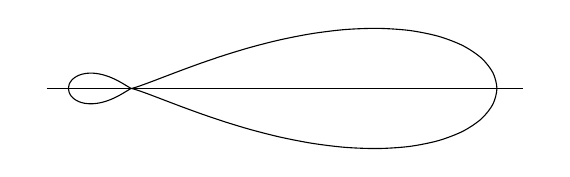
\begin{tikzpicture}
   \draw plot[
          variable=\t,
          domain=0:360,
          smooth,samples=51
      ] 
    ({20*sin(\t)}:{6*pow(0.95*sin(\t/2),5)});
  
   \draw plot[
          variable=\t,
          domain=0:360,
          smooth,samples=51
      ] 
    ({180+30*sin(\t)}:{0.8*pow(sin(\t/2),5)});

  \draw(-1.2,0) node[] (A) {};
  \draw( 5.1,0) node[] (B) {};
  
  \draw[] (A.east)  -- (B.west);

\end{tikzpicture}
\end{document}
